\documentclass[a4paper,12pt]{article}
\usepackage[unicode,verbose]{hyperref}
\usepackage{amsmath,amssymb,amsthm} 
\usepackage{pb-diagram}
\usepackage{ucs}
%\usepackage[utf8x]{inputenc}
%\usepackage[russian]{babel}
\usepackage{cmap}
\usepackage[pdftex]{graphicx}
\pagestyle{plain}
\theoremstyle{definition} \newtheorem{Def}{Definition}
%\usepackage{verbatim} 
\newenvironment{comment}
{\par\noindent{\bf TODO}\\}
{\\\hfill$\scriptstyle\blacksquare$\par}

\begin{document}
\title{\textbf{{\Large {Recurrent relation for branching coefficients of affine Lie algebras}}}}
\author{Vladimir Lyakhovsky\\
Theoretical Department, SPb State University,\\
198904, Sankt-Petersburg, Russia \\
e-mail:lyakh1507@nm.ru \\
[5mm] Anton Nazarov \\
%EndAName
Theoretical Department, SPb State University,\\
198904, Sankt-Petersburg, Russia \\
e-mail:antonnaz@gmail.com\\
}
\maketitle

\begin{abstract}
  We present the recurrent relation for the branching coefficients of affine Lie algebras. Then we describe the algorithm for the decomposition of  integrable highest weight modules
of a simple Lie algebra with respect to its reductive subalgebra which is based upon this recurrent relation and present some examples. Also we discuss the appearance of branching coefficients in the physical models.
\end{abstract}


\section{Introduction}
\label{sec:introduction}

The problem of the reduction of Lie algebra representation to the representations of the subalgebra is studied for several decades and has various applications in physics. In the context of finite-dimensional algebras it is important for the study of great unification models whilst the problem of the branching of the affine Lie algebras emerges in conformal field theory, for example, in the construction of the modular-invariant partition functions \cite{difrancesco1997cft}.

There exist several approaches to the computation of the branching coefficients which use the BGG
resolution \cite{bernstein1975differential} (for Kac-Moody algebras the algorithm is described in 
\cite{kac1990idl},\cite{wakimoto2001idl}), the Schure function series \cite{fauser2006new}, the BRST
cohomology \cite{hwang1994general}, Kac-Peterson formulas \cite{kac1990idl,quella2002branching} or the
combinatorial methods applied in \cite{feigin707principal}. 

Usually only the embedding of the maximal reductive subalgebras is considered since the case of non-maximal subalgebra can be obtained using the chain of maximal subalgebras. In this paper we present the recurrent formula for the branching coefficients which generalises the recurrent relation of the paper \cite{ilyin812pbc} to the case of non-maximal reductive subalgebra. Using this relation we formulate simple explicit algorithm for the computation of the branching coefficients which is applicable to the non-maximal subalgebras of finite-dimensional and affine Lie algebras.

We show that our algorithm can be used in the study of the conformal embeddings where the central charge of the conformal field theory is preserved, but the computation in this case is simplified using physical requirements.

The paper is organised as follows. In the next subsection of the introduction we fix the notation used throughout the paper. Then in Section \ref{sec:recurr-form-branch} we derive the central recurrent formula for the anomalous branching coefficients and describe the algorithm for the decomposition of the integrable highest weight modules of algebra $\mathfrak{g}$ to the modules of a reductive subalgebra $\mathfrak{a}$ (subsection \ref{sec:algorithm}). In the next Section \ref{sec:examples} we present several examples and discuss some applications in the physical models (s. \ref{sec:phys-appl}). We conclude the paper with the review of results and discussion of possible future developments (s. \ref{sec:conclusion}).

\subsection{Notation}
\label{sec:notation}

Consider affine Lie algebras $\frak{g}$ and $\frak{a}$ with the
underlying finite-dimensional subalgebras $\overset{\circ }{\frak{g}}$ and $%
\overset{\circ }{\frak{a}}$ and an injection $\frak{a}\longrightarrow \frak{g%
}$ such that $\frak{a}$ is a reductive subalgebra $\frak{a\subset g}$ with
correlated root spaces: $\frak{h}_{\frak{a}}^{\ast }\subset \frak{h}_{\frak{g%
}}^{\ast }$ and $\frak{h}_{\overset{\circ }{\frak{a}}}^{\ast }\subset \frak{h%
}_{\overset{\circ }{\frak{g}}}^{\ast }$\ .

We use the following notations adopted from the paper \cite{ilyin812pbc}.

$L^{\mu }$\ $\left( L_{\frak{a}}^{\nu }\right) $\ --- the integrable module
of $\frak{g}$ with the highest weight $\mu $\ ; (resp. integrable $\frak{a}$
-module with the highest weight $\nu $ );

$r$ , $\left( r_{\frak{a}}\right) $ --- the rank of the algebra $\frak{g}$ $%
\left( \text{resp. }\frak{a}\right) $ ;

$\Delta $ $\left( \Delta _{\frak{a}}\right) $--- the root system; $\Delta
^{+} $ $\left( \text{resp. }\Delta _{\frak{a}}^{+}\right) $--- the positive
root system (of $\frak{g}$ and $\frak{a}$ respectively);

$\mathrm{mult}\left( \alpha \right) $ $\left( \mathrm{mult}_{\frak{a}}\left(
\alpha \right) \right) $ --- the multiplicity of the root $\alpha$ in $\Delta 
$ (resp. in $\left( \Delta _{\frak{a}}\right) $);

$\overset{\circ }{\Delta }$ , $\left( \overset{\circ }{\Delta _{\frak{a}}}%
\right) $ --- the finite root system of the subalgebra $\overset{\circ }{%
\frak{g}}$ (resp. $\overset{\circ }{\frak{a}}$);

$\mathcal{N}^{\mu }$ , $\left( \mathcal{N}_{\frak{a}}^{\nu }\right) $ --- the
weight diagram of $L^{\mu }$ $\left( \text{resp. }L_{\frak{a}}^{\nu }\right) 
$ ;

$W$ , $\left( W_{\frak{a}}\right) $--- the corresponding Weyl group;

$C$ , $\left( C_{\frak{a}}\right) $--- the fundamental Weyl chamber;

$\bar{C}, \left(\bar{C_{\mathfrak{a}}}\right)$ --- the closure of the fundamental Weyl chamber;

$\rho $\ , $\left( \rho _{\frak{a}}\right) $\ --- the Weyl vector;

$\epsilon \left( w\right) :=\det \left( w\right) $ ;

$\alpha _{i}$ , $\left( \alpha _{\left( \frak{a}\right) j}\right) $ --- the $i
$-th (resp. $j$-th) basic root for $\frak{g}$ $\left( \text{resp. }\frak{a}%
\right) $; $i=0,\ldots ,r$ ,\ \ $\left( j=0,\ldots ,r_{\frak{a}}\right) $;

$\delta $ --- the imaginary root of $\frak{g}$ (and of $\frak{a}$ if any);

$\alpha _{i}^{\vee }$ , $\left( \alpha _{\left( \frak{a}\right) j}^{\vee
}\right) $--- the basic coroot for $\frak{g}$ $\left( \text{resp. }\frak{a}%
\right) $ , $i=0,\ldots ,r$ ;\ \ $\left( j=0,\ldots ,r_{\frak{a}}\right) $;

$\overset{\circ }{\xi }$ , $\overset{\circ }{\xi _{\left( \frak{a}\right) }}$
--- the finite (classical) part of the weight $\xi \in P$ , $\left( \text{%
resp. }\xi _{\left( \frak{a}\right) }\in P_{\frak{a}}\right) $;

$\lambda =\left( \overset{\circ }{\lambda };k;n\right) $ --- the
decomposition of an affine weight indicating the finite part $\overset{\circ 
}{\lambda }$, level $k$ and grade $n$\ .

$P$ $\left( \text{resp. } P_{\frak{a}}\right) $ \ --- the weight lattice;

$M \left( \text{resp. }M_{\frak{a}}\right) :=$

\noindent $=\left\{ 
\begin{array}{c}
\sum_{i=1}^{r}\mathbf{Z}\alpha _{i}^{\vee }\text{ }\left( \text{resp. }%
\sum_{i=1}^{r}\mathbf{Z}\alpha _{\left( \frak{a}\right) i}^{\vee }\right) 
\text{for untwisted algebras or }A_{2r}^{\left( 2\right) }, \\ 
\sum_{i=1}^{r}\mathbf{Z}\alpha _{i}\text{ }\left( \text{resp. }\sum_{i=1}^{r}%
\mathbf{Z}\alpha _{\left( \frak{a}\right) i}\right) \text{for }A_{r}^{\left(
u\geq 2\right) }\text{ and }A\neq A_{2r}^{\left( 2\right) },
\end{array}
\right\} ;$
$\Psi ^{\left( \mu \right) }:=\sum\limits_{w\in W}\epsilon (w)e^{w\circ (\mu +\rho )-\rho }$ --- the singular weight element for the $\frak{g}$-module $L^{\mu }$;
$\Psi _{\left( \frak{a}\right) }^{\left( \nu \right) }:=\sum\limits_{w\in W_{\frak{a}}}\epsilon (w)e^{w\circ (\nu +\rho
_{_{\frak{a}}})-\rho _{_{\frak{a}}}}$ --- the corresponding singular weight
element for the $\frak{a}$-module $L_{\frak{a}}^{\nu }$;

$\widehat{\Psi ^{\left( \mu \right) }}$ $\left( \widehat{\Psi _{\left( \frak{%
a}\right) }^{\left( \nu \right) }}\right) $ --- the set of singular weights $%
\xi \in P$ $\left( \text{resp. }\in P_{\frak{a}}\right) $ for the module $%
L^{\mu }$ $\left( \text{resp. }L_{\frak{a}}^{\nu }\right) $ with the
coordinates $\left( \overset{\circ }{\xi },k,n,\epsilon \left( w\left( \xi
\right) \right) \right) \mid _{\xi =w\left( \xi \right) \circ (\mu +\rho
)-\rho },$ (resp. $\left( \overset{\circ }{\xi },k,n,\epsilon \left(
w_{a}\left( \xi \right) \right) \right) \mid _{\xi =w_{a}\left( \xi \right)
\circ (\nu +\rho _{a})-\rho _{a}}$ ), (this set is similar to $P_{\mathrm{%
nice}}^{\prime }\left( \mu \right) $ in \cite{wakimoto2001idl})

$m_{\xi }^{\left( \mu \right) }$ , $\left( m_{\xi }^{\left( \nu \right)
}\right) $ --- the multiplicity of the weight $\xi \in P$ \ $\left( \text{%
resp. }\in P_{\frak{a}}\right) $ in the module $L^{\mu }$ , (resp. $\xi \in
L_{\frak{a}}^{\nu } $);

$ch\left( L^{\mu }\right) $ $\left( \text{resp. }ch\left( L_{\frak{a}}^{\nu
}\right) \right) $--- the formal character of $L^{\mu }$ $\left( \text{resp. }%
L_{\frak{a}}^{\nu }\right) $;

$ch\left( L^{\mu }\right) =\frac{\sum_{w\in W}\epsilon (w)e^{w\circ (\mu
+\rho )-\rho }}{\prod_{\alpha \in \Delta ^{+}}\left( 1-e^{-\alpha }\right) ^{%
\mathrm{{mult}\left( \alpha \right) }}}=\frac{\Psi ^{\left( \mu \right) }}{%
\Psi ^{\left( 0\right) }}$ --- the Weyl-Kac formula.

$R:=\prod_{\alpha \in \Delta ^{+}}\left( 1-e^{-\alpha }\right) ^{\mathrm{{%
mult}\left( \alpha \right) }}=\Psi ^{\left( 0\right) }\quad $

\noindent $\left( \text{resp. }R_{\frak{a}}:=\prod_{\alpha \in \Delta _{%
\frak{a}}^{+}}\left( 1-e^{-\alpha }\right) ^{\mathrm{mult}_{\frak{a}}\mathrm{%
\left( \alpha \right) }}=\Psi _{\frak{a}}^{\left( 0\right) }\right) $--- the
denominator.

$  L_{\frak{g}\downarrow \frak{a}}^{\mu }=\bigoplus\limits_{\nu \in P_{\frak{a}}^{+}}b_{\nu }^{\left( \mu \right) }L_{\frak{a}}^{\nu }$ --- the reduction of the representation;


$b^{(\mu)}_{\nu}$ --- the branching coefficients;

\begin{equation}
  \label{eq:21}
  \sum_{\nu \in \bar{C_{\mathfrak{a}}}}b_{\nu }^{\left( \mu \right) }\Psi _{\left( \frak{%
        a}\right) }^{\left( \nu \right) }=\sum_{\lambda \in P_{\frak{a}}}k_{\lambda
  }^{\left( \mu \right) }e^{\lambda } 
\end{equation}

 $k_{\lambda}$ --- the anomalous branching coefficients;

It is important to mention that
\begin{equation}
  \label{eq:20}
  b^{(\mu)}_{\nu}=k^{(\mu)}_{\nu} \; \mbox{for} \; \nu\in \bar{C}_{\mathfrak{a}}
\end{equation}

\section{Recurrent relation for branching coefficients}
\label{sec:recurr-form-branch}

Here we present the final recurrent relation for the anomalous branching coefficients \eqref{eq:21}. 
\begin{equation}
  \label{eq:1}
k_{\xi }^{\left( \mu \right) }=-\frac{1}{s\left( \gamma _{0}\right) }\left(
  \sum_{\omega\in W_{\bot}\backslash W} \epsilon(\omega)\; {\rm dim}\left(L^{\pi_{\mathfrak{a}_{\bot}}(\omega(\mu+\rho))-\rho_{\mathfrak{a}_{\bot}}}_{\mathfrak{a}_{\bot}}\right) \delta_{\xi-\gamma_0,\pi_{\mathfrak{a}}(\omega(\mu+\rho)-\rho)}+
\sum_{\gamma \in
\Gamma _{\frak{a}\subset \frak{g}}}s\left( \gamma +\gamma _{0}\right) k_{\xi
+\gamma }^{\left( \mu \right) }\right)   
\end{equation}
The proof of the formula and definitions of $\mathfrak{a}_{\bot},\; W_{\bot},\; s(\gamma),\; \Gamma_{\mathfrak{a}\subset \mathfrak{g}}$ are in the following subsection.

In the next section we describe the algorithm for the computation of branching coefficients based upon this formula and then present some example and discuss physical meaning.
\begin{comment}
  Fix the relation so that the definitions are available for the reader.
\end{comment}
\subsection{Proof of the recurrent relation}
\label{sec:proof}

The decomposition of the representation of the algebra to the representations of the subalgebra can be symbolically written using formal characters and projection operator $\pi_{\mathfrak{a}}$ to the weight subspace:
\begin{equation}
  \label{eq:3}
  L_{\frak{g}\downarrow \frak{a}}^{\mu }=\bigoplus\limits_{\nu \in P_{\frak{a}%
    }^{+}}b_{\nu }^{\left( \mu \right) }L_{\frak{a}}^{\nu }\quad
  \Longrightarrow\quad
  \pi_{\mathfrak{a}}(ch L^{\mu}_{\mathfrak{g}})=\sum_{\nu\in P^{+}_{\mathfrak{a}}}b^{(\mu)}_{\nu} ch L^{\nu}_{\mathfrak{a}}
\end{equation}
Using the Weyl-Kac formula for the character of the module
we obtain the equality
\begin{equation}
  \label{eq:4}
  \pi_{\mathfrak{a}}\left(\frac{\sum_{\omega\in W} \epsilon(\omega) e^{\omega(\mu+\rho)-\rho}}{\prod_{\alpha\in\Delta^{+}}(1-e^{-\alpha})^{\mathrm{mult}(\alpha)}}\right) = 
  \sum_{\nu\in P^{+}_{\mathfrak{a}}}b^{(\mu)}_{\nu}
  \frac{\sum_{\omega\in W_{\mathfrak{a}}}\epsilon(\omega)e^{\omega(\nu+\rho_{\mathfrak{a}})-\rho_{\mathfrak{a}}}}{\prod_{\beta\in \Delta_{\mathfrak{a}}^{+}}(1-e^{-\beta})^{\mathrm{mult}_{\mathfrak{a}}(\beta)}}
\end{equation}

It is important to mention that the projection of some of the positive roots of the algebra $\mathfrak{g}$ can be equal to zero. These roots are orthogonal to the root space of the subalgebra $\mathfrak{a}$ embedded into the root space of the algebra $\mathfrak{g}$. Let's denote the subset of these roots by $\Delta^{+}_{\bot}=\left\{\alpha\in\Delta_{\mathfrak{g}}^{+}:\forall \beta\in \Delta_{\mathfrak{a}}^{+},\; \alpha\bot\beta \right\}$.

We should notice that if the set $\Delta^{+}_{\bot}$ is non-empty than Weyl reflections which correspond to the positive roots of $\Delta^{+}_{\bot}$ generate a subgroup $W_{\bot}$ of Weyl group $W$. Consider any two positive roots $\alpha,\; \beta\in \Delta^{+}_{\bot}$ and corresponding Weyl reflections $\omega_{\alpha},\; \omega_{\beta}\in W_{\bot}$.  Since roots of the subalgebra $\mathfrak{a}$ are invariant under $\omega_{\alpha}, \; \omega_{\beta}$ they are also invariant under the action of $\omega_{\gamma}=\omega_{\alpha}\cdot \omega_{\beta}$. So the subgroup $W_{\bot}$ preserves the root system of the subalgebra $\mathfrak{a}$. 

The action of the Weyl subgroup $W_{\bot}$ on the set $\Delta^{+}_{\bot}$ produce the root system $\Delta_{\bot}$ which is orthogonal to the root system $\Delta_{\mathfrak{a}}$ of the subalgebra $\mathfrak{a}$. This root system can be considered as the root system of some subalgebra $\mathfrak{a}_{\bot}\subset \mathfrak{g}$.

Now we should discuss when the subset $\Delta^{+}_{\bot}$ is non-empty and the subgroup $W_{\bot}$ and subalgebra $\mathfrak{a}_{\bot}$ are non-trivial.
\begin{comment}
  Rewrite the following paragraph so that the limit is correct. Add the formula from the paper \cite{ilyin812pbc} here or near the recurrent relation (\ref{eq:1}).
\end{comment}
If $\mathfrak{a}$ is a maximal regular subalgebra of $\mathfrak{g}$ then rank of $\mathfrak{a}$ is equal to the rank of $\mathfrak{g}$ and it is clear that $\Delta^{+}_{\bot}$ is empty.
Then the modules $L_{\mathfrak{a}_{\bot}}$ are trivial, the dimensions are equal to 1 and we get the formula (11) from the paper \cite{ilyin812pbc}.
\begin{comment}
  Analyze all the regular embeddings and show when there exist orthogonal roots 
\end{comment}
Non-maximal regular embedding of $\mathfrak{a}$ into $\mathfrak{g}$ can be obtained through the chain of maximal embeddings $\mathfrak{a}\subset \mathfrak{p}_1\subset \mathfrak{p}_2\subset\dots \subset \mathfrak{g}$. Also the maximal regular embeddings are constructed by the exclusion of one or two roots from the extended Dynkin diagram of the algebra. Since this process can give us non-connected Dynkin diagrams we can see which roots are orthogonal to the root space of non-maximal regular subalgebra $\mathfrak{a}$. 

Consider for example regular embedding of $A_1\subset B_2$ ($su(2)\subset so(5)$). 

The extended Dynkin diagram of $B_2$ 
\begin{figure}[ph]
  \centering
  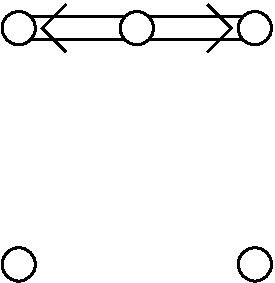
\includegraphics[width=40mm]{B2_A1_diagram.pdf}
  \caption{Extended Dynkin diagram of $B_2$ and embedding of $A_1$}
  \label{fig:B2Dynkin}
\end{figure}
We then drop central node and get the embedding $A_1\oplus A_1\subset B_2$. Then $\mathfrak{a}=A_1$ and $\mathfrak{a}_{\bot}=A_1$.
\begin{comment}
  Add the embedding index to the definitions
\end{comment}
In the case of special embeddings the set $\Delta^{+}_{\bot}$ can be empty as for the special embedding of $A_1\subset A_2$ with the embedding index equal to 4, or non-empty for example for the embedding $su(p)\subset su(p)\oplus su(q)\subset $
\begin{comment}
  Add here the example
\end{comment}


We can multiply the equation (\ref{eq:4}) by the term
\begin{equation}
  \label{eq:5}
  \pi_{\mathfrak{a}}\left(\prod_{\alpha\in \Delta^{+}\setminus \Delta^{+}_{\bot}}(1-e^{-\alpha})^{\mathrm{mult}_{\mathfrak{g}}(\alpha)} \right)
\end{equation}
This term is non-zero. 

Also we can see that for any formal polynomial or series $Q$
\begin{equation}
  \label{eq:6}
  \pi_{\mathfrak{a}} (Q) \pi_{\mathfrak{a}}(1-e^{-\alpha})=\pi_{\mathfrak{a}}\left(Q\cdot (1-e^{-\alpha})\right)
\end{equation}

The equation (\ref{eq:4}) takes the form
\begin{multline}
  \label{eq:7}
  \pi_{\mathfrak{a}}\left(\frac{\sum_{\omega\in W} \epsilon(\omega) e^{\omega(\mu+\rho)-\rho}}{\prod_{\alpha\in\Delta^{+}_{\bot}}(1-e^{-\alpha})^{\mathrm{mult}(\alpha)}}\right) = \\
  \pi_{\mathfrak{a}}\left(\prod_{\alpha\in \Delta^{+}\setminus \Delta^{+}_{\bot}}(1-e^{-\alpha})^{\mathrm{mult}_{\mathfrak{g}}(\alpha)} \right)\sum_{\nu\in P^{+}_{\mathfrak{a}}}b^{(\mu)}_{\nu}
  \frac{\sum_{\omega\in W_{\mathfrak{a}}}\epsilon(\omega)e^{\omega(\nu+\rho_{\mathfrak{a}})-\rho_{\mathfrak{a}}}}{\prod_{\beta\in \Delta_{\mathfrak{a}}^{+}}(1-e^{-\beta})^{\mathrm{mult}_{\mathfrak{a}}(\beta)}}
\end{multline}
The right-hand side of this equation can be reorganised as in the paper \cite{ilyin812pbc}. We introduce the anomalous branching coefficients $k_{\lambda}$.
\begin{equation}
  \label{eq:10}
  \sum_{\nu \in P_{\frak{a}}}b_{\nu }^{\left( \mu \right) }\Psi _{\left( \frak{%
        a}\right) }^{\left( \nu \right) }=\sum_{\lambda \in P_{\frak{a}}}k_{\lambda
  }^{\left( \mu \right) }e^{\lambda } 
\end{equation}
Also we extract the common denominator of  the right-hand side of the equation (\ref{eq:7})
\begin{multline}
  \label{eq:12}
  \pi_{\mathfrak{a}}\left(\frac{\sum_{\omega\in W} \epsilon(\omega) e^{\omega(\mu+\rho)-\rho}}{\prod_{\alpha\in\Delta^{+}_{\bot}}(1-e^{-\alpha})^{\mathrm{mult}(\alpha)}}\right) = \\
  \left(\prod_{\alpha\in \pi_{\mathfrak{a}}\left(\Delta^{+}\setminus \Delta^{+}_{\bot}\right)}(1-e^{-\alpha})^{{\rm mult}_{\mathfrak{g}}(\alpha)-{\rm mult}_{\mathfrak{\alpha}}} \right)
    \sum_{\lambda \in P_{\frak{a}}}k_{\lambda}^{\left( \mu \right) }e^{\lambda } 
\end{multline}


If the set $\Delta^{+}_{\bot}$ is non-empty then the Weyl reflections corresponding to the positive roots of $\Delta^{+}_{\bot}$ generate a subgroup $W_{\bot}$ of Weyl group $W$. 

We have denoted the subalgebra with the root space spanned over the set $\Delta^{+}_{\bot}$ by $\mathfrak{a}_{\bot}$.

Then we can reorganise the summation on the left-hand side of the equation (\ref{eq:12}) in the following way.
We consider the factor-group $W_{\bot}\backslash W$ and the left conjugate classes. For the class $\tilde{\omega}\in W_{\bot}\backslash W$ we choose the representative $\omega \in \tilde{\omega}$ in such a way that $\omega(\mu+\rho)\in \bar{C}_{\mathfrak{a}_{\bot}}$. Then
\begin{multline}
  \label{eq:13}
 \pi_{\mathfrak{a}}\left(\frac{\sum_{\omega\in W} \epsilon(\omega) e^{\omega(\mu+\rho)-\rho}}{\prod_{\alpha\in\Delta^{+}_{\bot}}(1-e^{-\alpha})^{\mathrm{mult}(\alpha)}}\right) = \\
 \pi_{\mathfrak{a}}\left(\sum_{\omega\in W_{\bot}\backslash W} \epsilon(\omega) \frac{\sum_{\nu\in W_{\bot}}\epsilon(\nu) e^{\nu \cdot \omega(\mu+\rho)-\rho}}{\prod_{\alpha\in\Delta^{+}_{\bot}}(1-e^{-\alpha})^{\mathrm{mult}(\alpha)}}\right) 
\end{multline}

We see that the fraction on the right-hand side of the equation looks like the character of some representation of the algebra $\mathfrak{a}_{\bot}$. 
In order to write it explicitly we rewrite $\nu\cdot\omega(\mu+\rho)-\rho$ as
\begin{equation}
  \label{eq:30}
  \nu\cdot\omega(\mu+\rho)-\rho=\nu\cdot \bigl(\omega(\mu+\rho)-\pi_{\mathfrak{a}}(\omega(\mu+\rho))-\rho_{\mathfrak{a}_{\bot}}+\rho_{\mathfrak{a}_{\bot}}+\pi_{\mathfrak{a}}(\omega(\mu+\rho))\bigr)-\rho
\end{equation}

Since $\nu\cdot \pi_{\mathfrak{a}}(\omega(\mu+\rho))=\pi_{\mathfrak{a}}(\omega(\mu+\rho))$ and $\omega(\mu+\rho)-\pi_{\mathfrak{a}}(\omega(\mu+\rho))=\pi_{\mathfrak{a}_{\bot}}(\omega(\mu+\rho))$, we get
\begin{multline}
  \label{eq:14}
  \sum_{\omega\in W_{\bot}\backslash W} \epsilon(\omega) \frac{\sum_{\nu\in W_{\bot}}\epsilon(\nu) e^{\nu \cdot \omega(\mu+\rho)-\rho}}{\prod_{\alpha\in\Delta^{+}_{\bot}}(1-e^{-\alpha})^{\mathrm{mult}(\alpha)}} =\\
  \sum_{\omega\in W_{\bot}\backslash W} \epsilon(\omega) e^{\pi_{\mathfrak{a}}(\omega(\mu+\rho))-\rho} \frac{e^{\rho_{\mathfrak{a}_{\bot}} }\sum_{\nu\in W_{\bot}}\epsilon(\nu) e^{\nu \cdot (\pi_{\mathfrak{a}_{\bot}}(\omega(\mu+\rho))-\rho_{\mathfrak{a}_{\bot}}+\rho_{\mathfrak{a}_{\bot}})-\rho_{\mathfrak{a}_{\bot}}}}{\prod_{\alpha\in\Delta^{+}_{\bot}}(1-e^{-\alpha})^{\mathrm{mult}(\alpha)}}=\\
  \sum_{\omega\in W_{\bot}\backslash W} \epsilon(\omega) e^{\pi_{\mathfrak{a}}(\omega(\mu+\rho))-\rho}e^{\rho_{\mathfrak{a}_{\bot}}} ch L^{\pi_{\mathfrak{a}_{\bot}}(\omega(\mu+\rho))-\rho_{\mathfrak{a}_{\bot}}}_{\mathfrak{a}_{\bot}}
\end{multline}
The projection $\pi_{\mathfrak{a}}$ of the character of the highest-weight module $L^{\pi_{\mathfrak{a}_{\bot}}(\omega(\mu+\rho))-\rho_{\mathfrak{a}_{\bot}}}_{\mathfrak{a}_{\bot}}$ is equal to the dimension of the module multiplied by the unity of the algebra of formal exponents. So we have
  \begin{multline}
    \label{eq:15}
    \pi_{\mathfrak{a}}\left( \sum_{\omega\in W_{\bot}\backslash W} \epsilon(\omega) e^{\pi_{\mathfrak{a}}(\omega(\mu+\rho))-\rho}e^{\rho_{\mathfrak{a}_{\bot}}} ch L^{\pi_{\mathfrak{a}_{\bot}}(\omega(\mu+\rho))-\rho_{\mathfrak{a}_{\bot}}}_{\mathfrak{a}_{\bot}}\right) = \\
    \sum_{\omega\in W_{\bot}\backslash W} \epsilon(\omega)\; \mathrm{dim}\left(L^{\pi_{\mathfrak{a}_{\bot}}(\omega(\mu+\rho))-\rho_{\mathfrak{a}_{\bot}}}_{\mathfrak{a}_{\bot}}\right) e^{\pi_{\mathfrak{a}}(\omega(\mu+\rho)-\rho)}
  \end{multline}
These dimensions of the modules could be easily calculated using the Weyl formula.
\begin{comment}
  Rewrite it, so that the following paragraph begins the computation
\end{comment}
This explicit calculation to get the character of the $\mathfrak{a}_{\bot}$ representation can be thought as the calculation of the character of the $\mathfrak{a}_{\bot}\oplus \mathfrak{h}$-module with the highest weight $\omega(\mu+\rho)$, where $\mathfrak{h}$ is the Cartan subalgebra of $\mathfrak{g}$.

Thus we have the equality
\begin{multline}
  \label{eq:9}
  \sum_{\omega\in W_{\bot}\backslash W} \epsilon(\omega) dim\left(L^{\pi_{\mathfrak{a}_{\bot}}(\omega(\mu+\rho))-\rho_{\mathfrak{a}_{\bot}}}_{\mathfrak{a}_{\bot}}\right) e^{\pi_{\mathfrak{a}}(\omega(\mu+\rho)-\rho)}=\\
  \left(\prod_{\alpha\in \pi_{\mathfrak{a}}\left(\Delta^{+}\setminus \Delta^{+}_{\bot}\right)}(1-e^{-\alpha})^{{\rm mult}_{\mathfrak{g}}(\alpha)-{\rm mult}_{\mathfrak{\alpha}}} \right)
  \sum_{\lambda \in P_{\frak{a}}}k_{\lambda}^{\left( \mu \right) }e^{\lambda } 
\end{multline}

We can rewrite the multiplier of the right-hand side as in the paper \cite{ilyin812pbc}.
\begin{equation}
  \label{eq:11}
    \prod_{\alpha\in \pi_{\mathfrak{a}}\circ (\Delta^{+}\setminus \Delta^{+}_{\bot})} \left(1-e^{-\alpha}\right)^{\mathrm{mult}(\alpha)-\mathrm{mult}_{\mathfrak{a}}(\alpha)}=
     -\sum_{\gamma\in P_{\mathfrak{a}}} s(\gamma)e^{-\gamma}
\end{equation}

For the coefficient function $s\left( \gamma \right) $ define $\Phi _{\frak{a%
}\subset \frak{g}}\subset P_{\frak{a}}$ as its carrier: 
\begin{equation}
\Phi _{\frak{a}\subset \frak{g}}=\left\{ \gamma \in P_{\frak{a}}\mid s\left(
\gamma \right) \neq 0\right\} ;  \label{phi-d}
\end{equation}
\begin{equation}
\prod_{\alpha\in \pi_{\mathfrak{a}}\circ (\Delta^{+}\setminus \Delta^{+}_{\bot})}\left(1-e^{-\alpha }\right) ^{\mathrm{{mult}\left( \alpha \right) -{mult}_{\frak{a}}}\mathrm{\left( \alpha \right) }}=-\sum_{\gamma \in \Phi _{\frak{a}\subset 
\frak{g}}}s\left( \gamma \right) e^{-\gamma }.  \label{fan-d}
\end{equation}

So we get the equation
\begin{multline}
  \label{eq:16}
  \sum_{\omega\in W_{\bot}\backslash W} \epsilon(\omega) dim\left(L^{\pi_{\mathfrak{a}_{\bot}}(\omega(\mu+\rho))-\rho_{\mathfrak{a}_{\bot}}}_{\mathfrak{a}_{\bot}}\right) e^{\pi_{\mathfrak{a}}(\omega(\mu+\rho)-\rho)}=\\
  = -\sum_{\gamma \in \Phi _{\frak{a}\subset \frak{g}}} s\left( \gamma \right) e^{-\gamma }\sum_{\lambda \in P_{\frak{a}}}
  k_{\lambda }^{\left( \mu \right) }e^{\lambda } \\
  =-\sum_{\gamma \in \Phi _{\frak{a}\subset \frak{g}}}\sum_{\lambda \in P_{\frak{a}}}s\left( \gamma \right) k_{\lambda }^{\left( \mu \right)}e^{\lambda -\gamma }
\end{multline}
From the equality of the coefficients of the equal formal exponents we get
\begin{equation}
  \label{eq:17}
   \sum_{\omega\in W_{\bot}\backslash W} \epsilon(\omega) dim\left(L^{\pi_{\mathfrak{a}_{\bot}}(\omega(\mu+\rho))-\rho_{\mathfrak{a}_{\bot}}}_{\mathfrak{a}_{\bot}}\right) \delta_{\xi,\pi_{\mathfrak{a}}(\omega(\mu+\rho)-\rho)}+
   \sum_{\gamma \in \Phi _{\frak{a}\subset \frak{g}}} s(\gamma)\; k^{(\mu)}_{\xi+\gamma}=0;\quad \xi\in P_{\mathfrak{a}}
\end{equation}

To get the recurrent relation for the anomalous branching coefficients we should use the following procedure, introduced in the paper \cite{ilyin812pbc}.

Let $\gamma
_{0} $ be the lowest vector with respect to the natural ordering in $%
\overset{\circ }{\Delta _{\frak{a}}}$ in the lowest grade of $\Phi _{\frak{a}\subset \frak{g}}$. Decomposing the defining relation (\ref{fan-d}) 
\begin{equation}
  \label{eq:18}
  \prod_{\alpha\in \pi_{\mathfrak{a}}\circ (\Delta^{+}\setminus \Delta^{+}_{\bot})}\left(
    1-e^{-\alpha }\right) ^{\mathrm{{mult}\left( \alpha \right) -{mult}}_{\frak{a%
      }}\mathrm{\left( \alpha \right) }}=-s\left( \gamma _{0}\right) e^{-\gamma
    _{0}}-\sum_{\gamma \in \Phi _{\frak{a}\subset \frak{g}}\setminus \left\{\gamma_{0}\right\}}s\left( \gamma \right) e^{-\gamma },  
\end{equation}
in (\ref{eq:17}) we obtain

\begin{equation}
  k_{\xi }^{\left( \mu \right) }=
  -\frac{1}{s\left( \gamma _{0}\right) }
  \left(
    \sum_{\omega\in W_{\bot}\backslash W} \epsilon(\omega)\; \mathrm{dim}
    \left(L^{\pi_{\mathfrak{a}_{\bot}}(\omega(\mu+\rho))-\rho_{\mathfrak{a}_{\bot}}}_{\mathfrak{a}_{\bot}}\right)
    \delta_{\xi-\gamma_0,\pi_{\mathfrak{a}}(\omega(\mu+\rho)-\rho)}+
    \sum_{\gamma \in \Gamma _{\frak{a}\subset \frak{g}}} s\left( \gamma +\gamma _{0}\right) k_{\xi+\gamma }^{\left( \mu \right) }
  \right)   
\label{recurrent relation}
\end{equation}
where the set 
\begin{equation}
\Gamma _{\frak{a}\subset \frak{g}}=\left\{ \xi -\gamma _{0}|\xi \in \Phi _{%
\frak{a}\subset \frak{g}}\right\} \setminus \left\{ 0\right\} .
\label{fan-defined}
\end{equation}

So we have obtained recurrent relation for the anomalous branching coefficients.  In the next section we describe the algorithm for the computation of branching coefficients using the relation \eqref{recurrent relation}. 

\subsection{Algorithm for the recursive computation of the branching coefficients}
\label{sec:algorithm}

We use the recurrent relation \eqref{recurrent relation} to formulate the algorithm for recursive computation of the branching coefficients. It is important to mention that the computation of the branching coefficients is organised without the  explicit construction of the module $L^{(\mu)}_{\mathfrak{g}}$ and any of the modules $L^{(\nu)}_{\mathfrak{a}}$. 

The algorithm is divided into the following steps.
\begin{enumerate}
\item Construct the set $\Delta^{+}$ of the positive roots of the algebra $\mathfrak{g}$.
\item Select the positive roots $\alpha\in \Delta^{+}$ which are orthogonal to the root subspace of the subalgebra $\mathfrak{a}$ and form the set $\Delta^{+}_{\bot}$.
\item Construct the set $\widehat{\Psi^{(\mu)}}=\left\{\omega(\mu+\rho)-\rho;\; \omega\in W\right\}$ of the anomalous points of the $\mathfrak{g}$-module $L^{(\mu)}$.
\item Select those weights $\lambda=\omega(\mu+\rho)$ which lies in the closure of the main Weyl chamber of the algebra $\mathfrak{a}_{\bot}$. Since we have constructed the set $\Delta^{+}_{\bot}$ we can easily check if the weight $\lambda$ lies in the main Weyl chamber of $\mathfrak{a}_{\bot}$ checking that the scalar product of $\lambda$ with the roots of $\Delta^{+}_{\bot}$ is non-negative.
\item For $\lambda=\omega(\mu+\rho),\; \lambda\in \bar{C}_{\mathfrak{a}_{\bot}}$ calculate the dimensions of the corresponding modules $\mathrm{dim}\left(L^{\pi_{\mathfrak{a}_{\bot}}(\omega(\mu+\rho))-\rho_{\mathfrak{a}_{\bot}}}_{\mathfrak{a}_{\bot}}\right)$ using the Weyl formula with the set $\Delta^{+}_{\bot}$.
\item Construct the set $\Gamma$ \eqref{fan-defined}.
\item Calculate anomalous branching coefficients in the main Weyl
  chamber of the subalgebra $\mathfrak{a}$ using recurrent relation (\ref{recurrent relation}).
\end{enumerate}

If we are interested in the branching coefficients for the embedding of the finite-dimensional Lie algebra into the affine Lie algebra we can construct the set of the anomalous points up to required grade and use steps 4-7 of the algorithm for each grade. We can also speed up the algorithm by one-time computation of the representatives of the conjugate classes $W_{\bot}\backslash W$.

The next section consists of several examples computed with this algorithm. 

\section{Examples}
\label{sec:examples}

\subsection{Finite dimensional Lie algebras}
\label{sec:finite-dimens-lie}

\subsubsection{Regular embedding of $A_1$ into $B_2$}
\label{sec:regul-embedd-a_1}

Consider the regular embedding of $A_1$ into $B_2$. Simple roots $\alpha_1, \alpha_2$ of $B_2$ are drawn as the thick vectors at the Figure \ref{fig:B2_A1}. We denote the corresponding Weyl reflections by $\omega_1, \omega_2$. Simple root $\beta$ of the embedded $A_1$ is equal to $\alpha_1+\alpha_2$.

Let's describe the reduction of fundamental representation of $B_2$ with the highest weight (in fundamental weight basis) equal to $(1,0)$.
\begin{figure}[ph]
  \noindent\centering{
    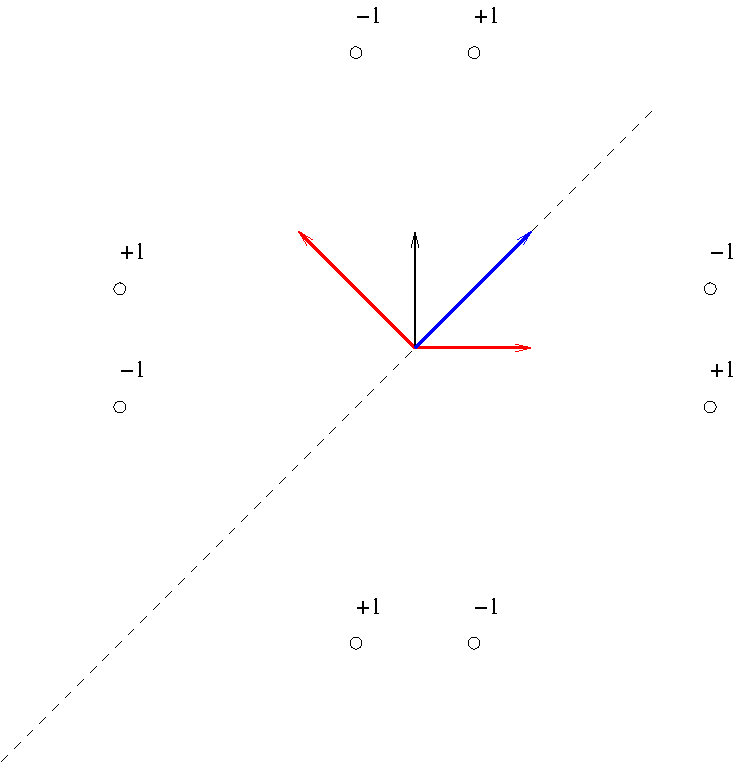
\includegraphics[width=90mm]{B2_A1.pdf}
  }
  \caption{Regular embedding of $A_1$ into $B_2$}
  \label{fig:B2_A1}
\end{figure}
On the Figure \ref{fig:B2_A1} we have also shown the set of points $\omega(\mu+\rho),\; \omega\in W$ of fundamental representation of $B_2$ with the corresponding determinants of Weyl reflections $\epsilon(\omega)$. 
Now we have to factorise the Weyl group $W$ by $W_{\bot}=\left\{\omega_1\right\}$. We get the following set of anomalous points $\omega(\mu+\rho)-\rho,\; \omega\in W_{\bot}\backslash W$:
\begin{figure}[ph]
  \noindent\centering{
    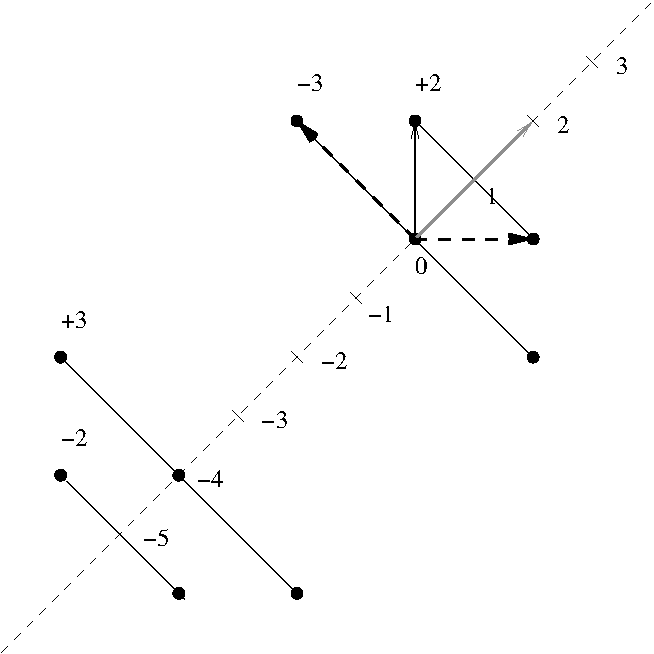
\includegraphics[width=90mm]{B2_A1_2.pdf}
  }
  \caption{Anomalous points and the corresponding $\mathfrak{a}_{\bot}=A_1$-modules}
  \label{fig:B2_A1_2}
\end{figure}
We have also depicted the corresponding $\mathfrak{a}_{\bot}=A_1$-modules $L^{\pi_{\mathfrak{a}_{\bot}}(\omega(\mu+\rho))-\rho_{\mathfrak{a}_{\bot}}}_{\mathfrak{a}_{\bot}}$.
Then we project these points and dimensions of modules onto the root space of subalgebra $\mathfrak{a}=A_1$ and get the following anomalous points in fundamental weights basis with corresponding multiplicities:
\begin{equation}
  \label{eq:25}
  (1,2),\; (0,-3),\; (-4,3),\; (-5,-2)
\end{equation}
For the function $s(\gamma)$ and the set $\Gamma$ from the definition (\ref{phi-d},\ref{fan-defined}) we have
\begin{equation}
  \label{eq:22}
  (0,1),\; (1,2),\; (2,-1)
\end{equation}
Here the second component denotes the value of $s(\gamma)$.
\begin{comment}
  It seems that here $\Gamma$ should include only two points. Is it true?

  Think of the pictures more.
\end{comment}
Anomalous branching coefficient $k^{(1,0)}_{1}=2$, then for anomalous branching coefficient $k^{(1,0)}_{0}$ the formula (\ref{recurrent relation}) gives us
\begin{equation}
  \label{eq:23}
  k^{(1,0)}_{0}=-1\cdot k^{(1,0)}_2 +2\cdot k^{(1,0}_1 - 3\cdot \delta_{0,0} = 1
\end{equation}
So we have computed the branching coefficients.
\subsubsection{Embedding of $B_2$ into $B_4$}
\label{sec:someth-high-dimens}
Consider the the regular embedding of the subalgebra $B_2$ into the algebra $B_4$.
We calculate the branching coefficients for the fundamental representation of $B_4$.
The corresponding Dynkin diagrams are in the Figure \ref{fig:dynkin}.
\begin{figure}[ph]
  \centering
  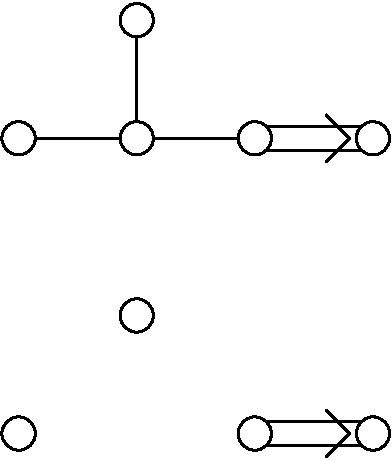
\includegraphics[width=60mm]{B4_B2_2A1.pdf}
  \caption{Dynkin diagrams}
  \label{fig:dynkin}
\end{figure}

In the orthogonal basis $e_1,\dots,e_4$ simple roots of $B_4$ are
\begin{equation}
  \label{eq:8}
  (e_1 - e_2,\; e_2 - e_3,\; e_3 - e_4,\; e_4)
\end{equation}
Positive roots are
\begin{multline}
  \label{eq:19}
  (e_1 - e_2,\; e_2 - e_3,\; e_3 - e_4,\; e_4,\; e_1 - e_3,\; e_2 - e_4,\; e_3 + e_4,\; e_3,\; e_1 - e_4,\;\\
    e_2 + e_4,\; e_2,\; e_1 + e_4,\; e_2 + e_3,\; e_1,\; e_1 + e_3,\; e_1 + e_2)
\end{multline}
Simple roots of the embedded subalgebra $\mathfrak{a}=B_2$ are
\begin{equation}
  \label{eq:26}
  (e_3-e_4,e_4)
\end{equation}

The set $\Delta^{+}_{\bot}$ is equal to
\begin{equation}
  \label{eq:27}
  \left\{e_1-e_2,e_1+e_2,e_1,e_2\right\}
\end{equation}

We see that this is the set of positive roots of the algebra $\mathfrak{a}_{\bot}=B_2$.

To find the branching coefficients we need to compute the anomalous points of $B_4$, select point lying in the main Weyl chamber of $\mathfrak{a}_{\bot}$ and compute the dimensions of corresponding $\mathfrak{a}_{\bot}$-modules.

We consider the $B_4$-module with the highest weight $\mu=(0,1,0,2)=2
e_1 + 2 e_2 + e_3 + e_4$.

The set of the anomalous points $\omega(\mu+\rho)-\rho,\; \omega\in W$
consists of 384 points. We do not show it here.

We need to select those points $\omega(\mu+\rho)$  which are projected into the main chamber of the embedded algebra $\mathfrak{a}_{\bot}$.
It means that scalar product of these points with all the roots from $\Delta^{+}_{\bot}$ is non-negative.

To compute dimensions of the corresponding
$\mathfrak{a}_{\bot}$-modules we need to project each selected point
onto the root space $\Delta^{+}_{\bot}$ and substract
$\rho_{\mathfrak{a}_{\bot}}$, then use Weyl dimension formula.

We show the result of this procedure on the Figure \ref{fig:B4B2anom}.
\begin{figure}[h]
    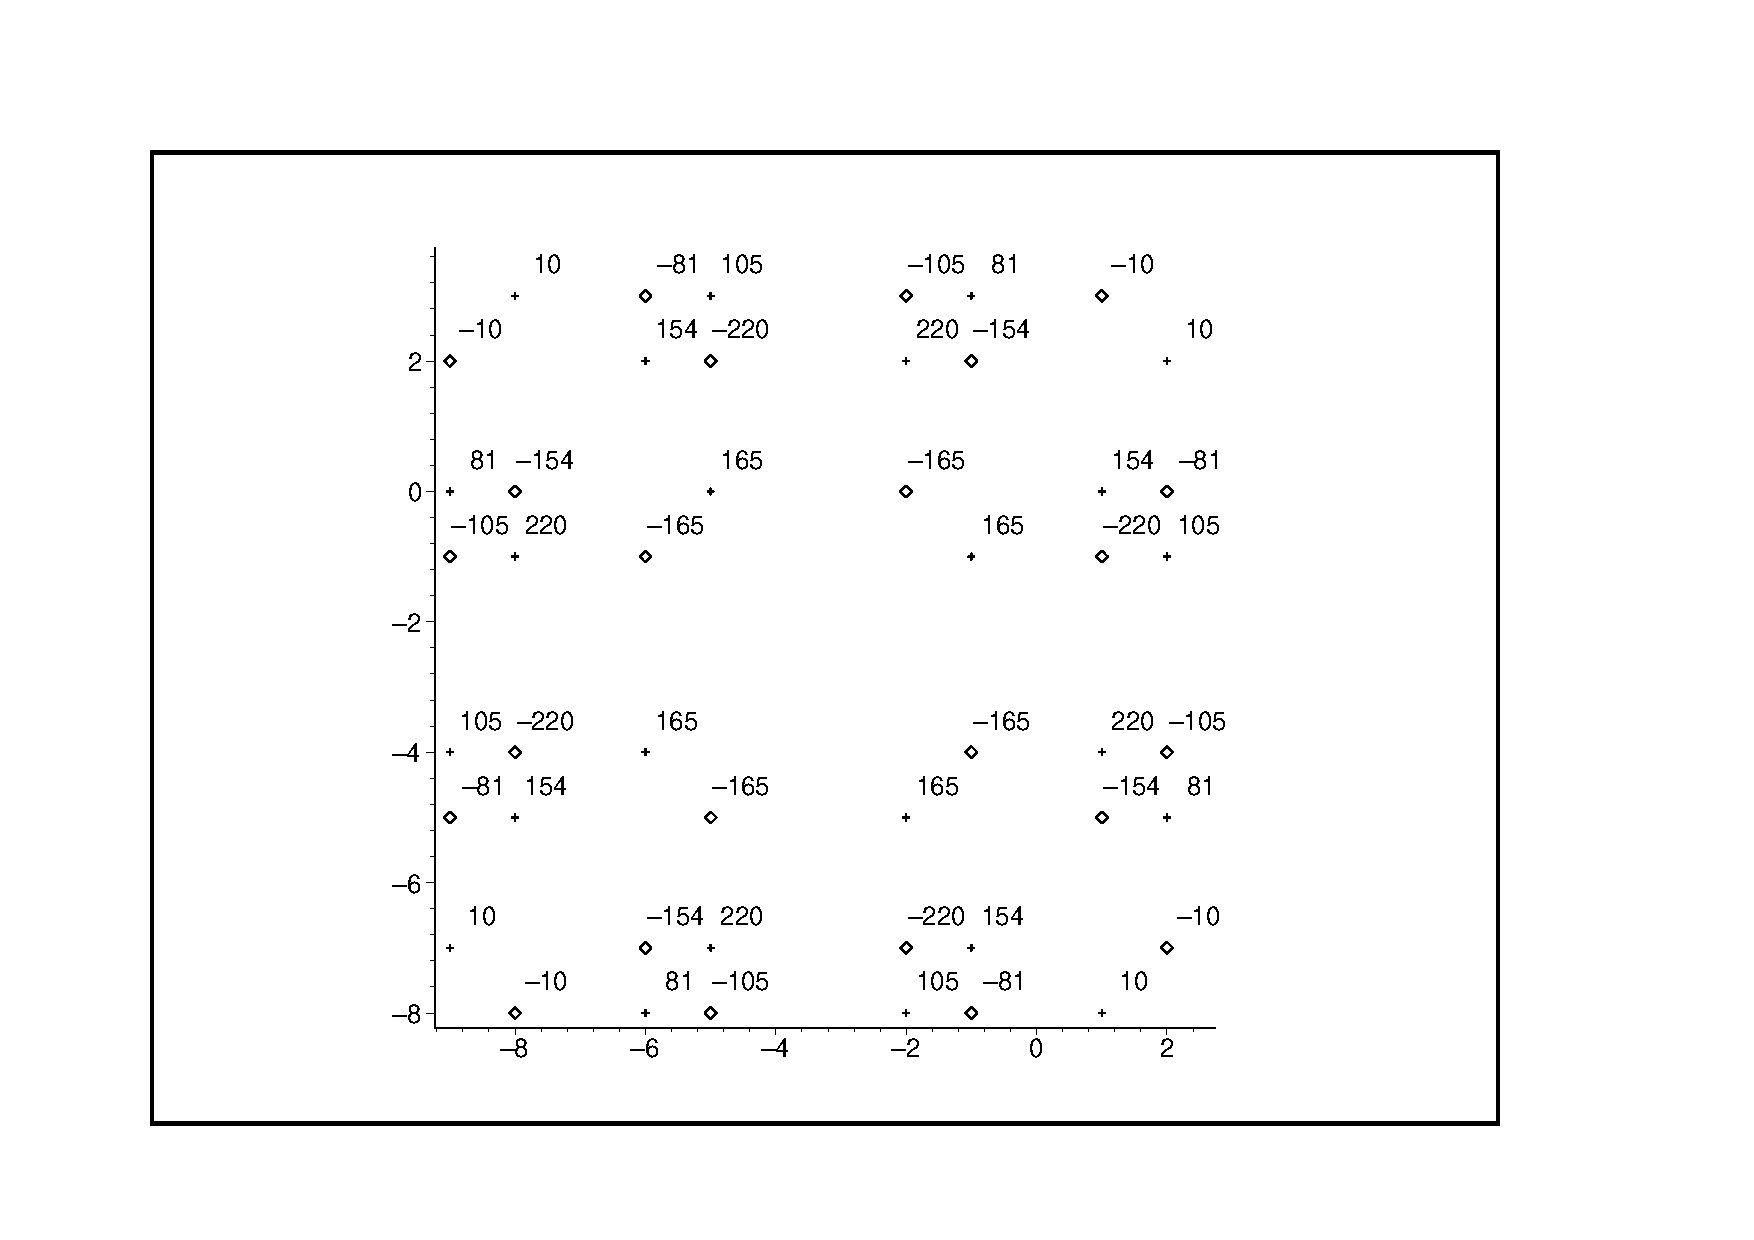
\includegraphics[width=170mm]{B4_B2_anom_points.pdf}
  \caption{Anomalous points with the dimensions of corresponding $\mathfrak{a}_{\bot}$-modules.}
  \label{fig:B4B2anom}
\end{figure}

Then we should construct ``the fan'' and use the recurrent relation for the computation of anomalous branching coefficients.

Using the definition (\ref{fan-defined}) we get the following set of
the points $\Gamma$ with the corresponding values $s(\gamma+\gamma_0)$
\begin{figure}[h]
  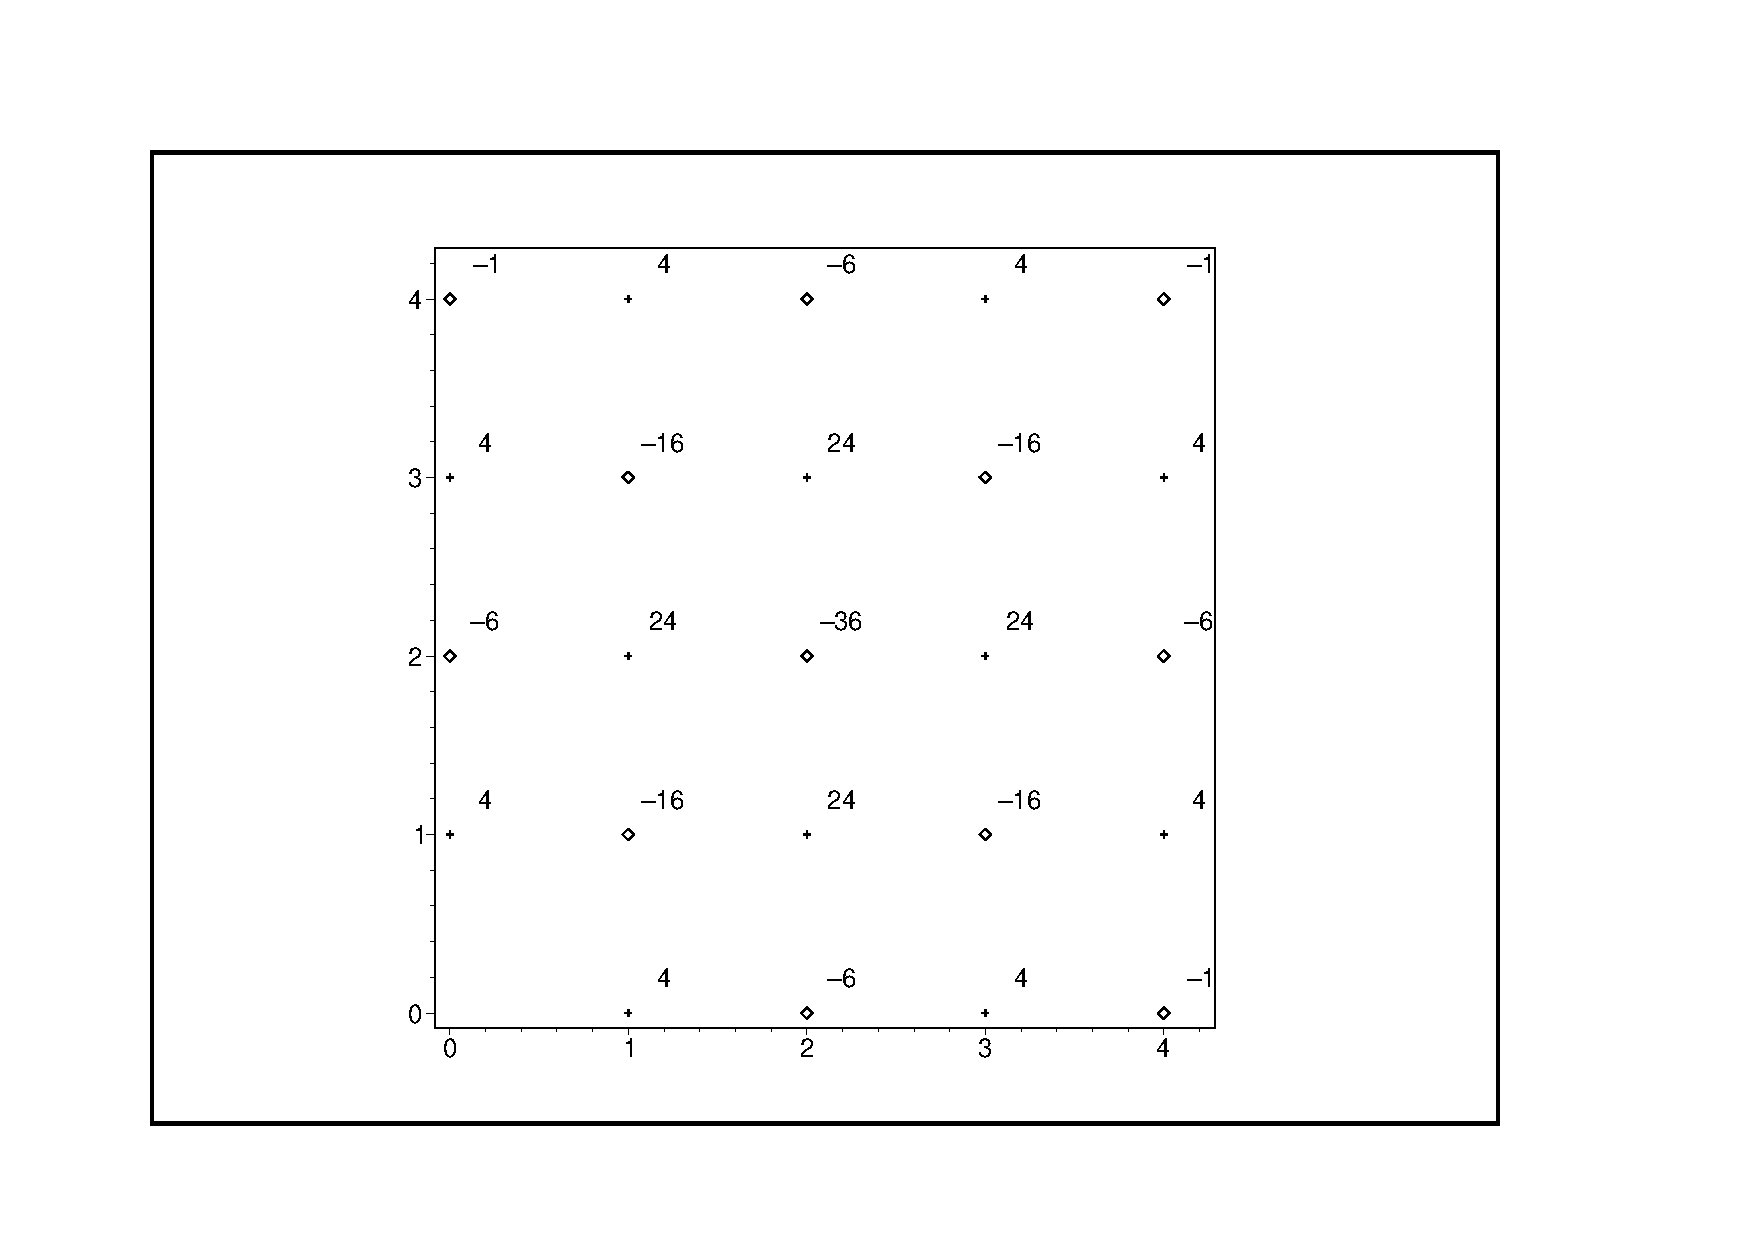
\includegraphics[width=150mm]{B4_B2_fan.pdf}
  \caption{Fan for $B_2\subset B_4$}
  \label{fig:B4B2Fan}
\end{figure}
We use the recurrent relation (\ref{recurrent relation}) and get
following branching coefficients:
\begin{equation}
  \label{eq:24}
  \pi_{\mathfrak{a}} \left(ch L^{(0,1,0,2)}_{B_4}\right) = 6 \; ch L^{(0,0)}_{B_2}+ 60
  \; ch L_{B_2}^{(0,2)}+ 30 \; ch L_{B_2}^{(1,0)}+ 19 \; ch L_{B_2}^{(2,0)}+
  40 \; ch L_{B_2}^{(1,2)}+ 10 \; ch L_{B_2}^{(2,2)}
\end{equation}
The dimension of the highest-weight $B_4$-module $L^{(0,1,0,2)}_{B_4}$
is equal to 2772. It is easy to see, that right-hand side of the
equation (\ref{eq:24}) gives the same result.

\subsection{Affine Lie algebras}
\label{sec:affine-lie-algebras}
%%  \subsubsection{Embedding of finite-dimensional algebra into affine algebra}
%%  \label{sec:embedd-finite-dimens}
%%  
%%  The maximal embeddings of the finite-dimensional Lie algebras into the affine Lie algebras were thoroughly studied and the tables of the branching coefficients are given in the book \cite{kass1990ala}. The task of the study of non-maximal embeddings is then can be reduced to the well-known task of branching of the finite-dimensional Lie algebras.
%%  Thus here we show the simplest possible example of reduction of affine $\hat{A_1}$ to $A_1$ in order to demonstrate some traits of our method and show that we eliminate the need of slice-by-slice study discussed in \cite{kass1990ala}.
%%  
%%  The simple roots for the affine $\hat{A_1}$ are
%%  \begin{equation}
%%    \label{eq:2}
%%    (\alpha,\delta-\alpha)
%%  \end{equation}
%%  We consider the embedding with the root $\beta=\delta-\alpha$. 
%%  
%%  Positive roots of the $\hat{A_1}$ are $\alpha,\; \alpha+n\delta,\; n\delta,\; -\alpha+n\delta;\; n=1,2,3,\dots$.
%%  The set of the 
%%  
\subsubsection{Embedding of the affine algebra into affine algebra}
\label{sec:embedd-affine-algebr}

Consider the affine extension of the example \ref{sec:regul-embedd-a_1}. 
Since this embedding is regular, the level of the representations of the subalgebra is equal to the level of the representation of the algebra. 

The set $\Delta^{+}_{\bot}$ of the orthogonal positive roots with the zero projection on the root space of the subalgebra $\hat{A_1}$ is the same as in the finite-dimensional case.

Consider the level one representation of the algebra $\mathfrak{g}=\hat{B_2}$ with the highest weight $w_1=(1,0,1,0)$, where the first to components are the coordinates of the classical part in the orthogonal basis $e_1,e_2$, the third is the grade of the weight and the fourth is the level.


The set of the anomalous points of this representation up to sixth grade is depicted in the Figure \ref{fig:affine_B2_anom_point} and in each grade it looks like in the Figure \ref{fig:B2_A1}. 

\begin{figure}[h!tb]
  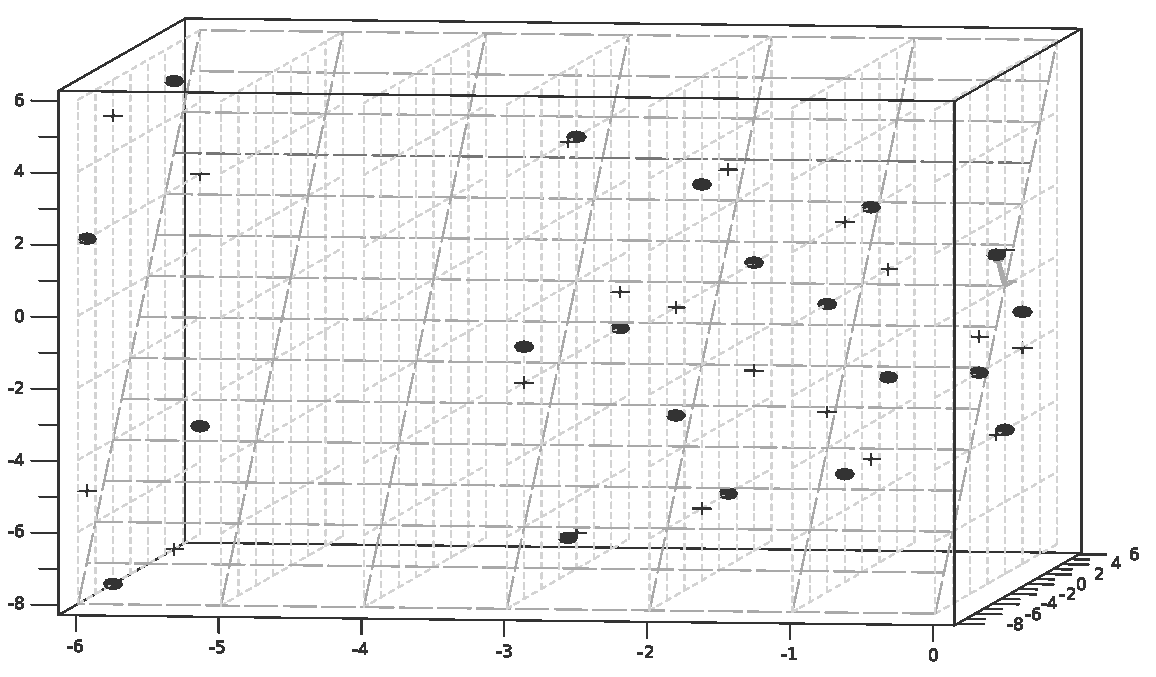
\includegraphics[width=160mm]{AffineB2_A1_Anom.pdf}
  \caption{The anomalous points of the $(1,0,1,0)$ representation of the algebra $\hat{B_2}$}
  \label{fig:affine_B2_anom_point}
\end{figure}

As the next step of our algorithm \ref{sec:algorithm} we project the anomalous points to the weight space of the subalgebra $\hat{A_1}$ and calculate the dimensions of the corresponding $\mathfrak{a}_{\bot}$-modules $L^{\pi_{\mathfrak{a}_{\bot}}(\omega(\mu+\rho))-\rho_{\mathfrak{a}_{\bot}}}_{\mathfrak{a}_{\bot}}$.
The result of this computation up to the twelfth grade is presented at the Figure
\begin{figure}[h!tb]
  \centering
  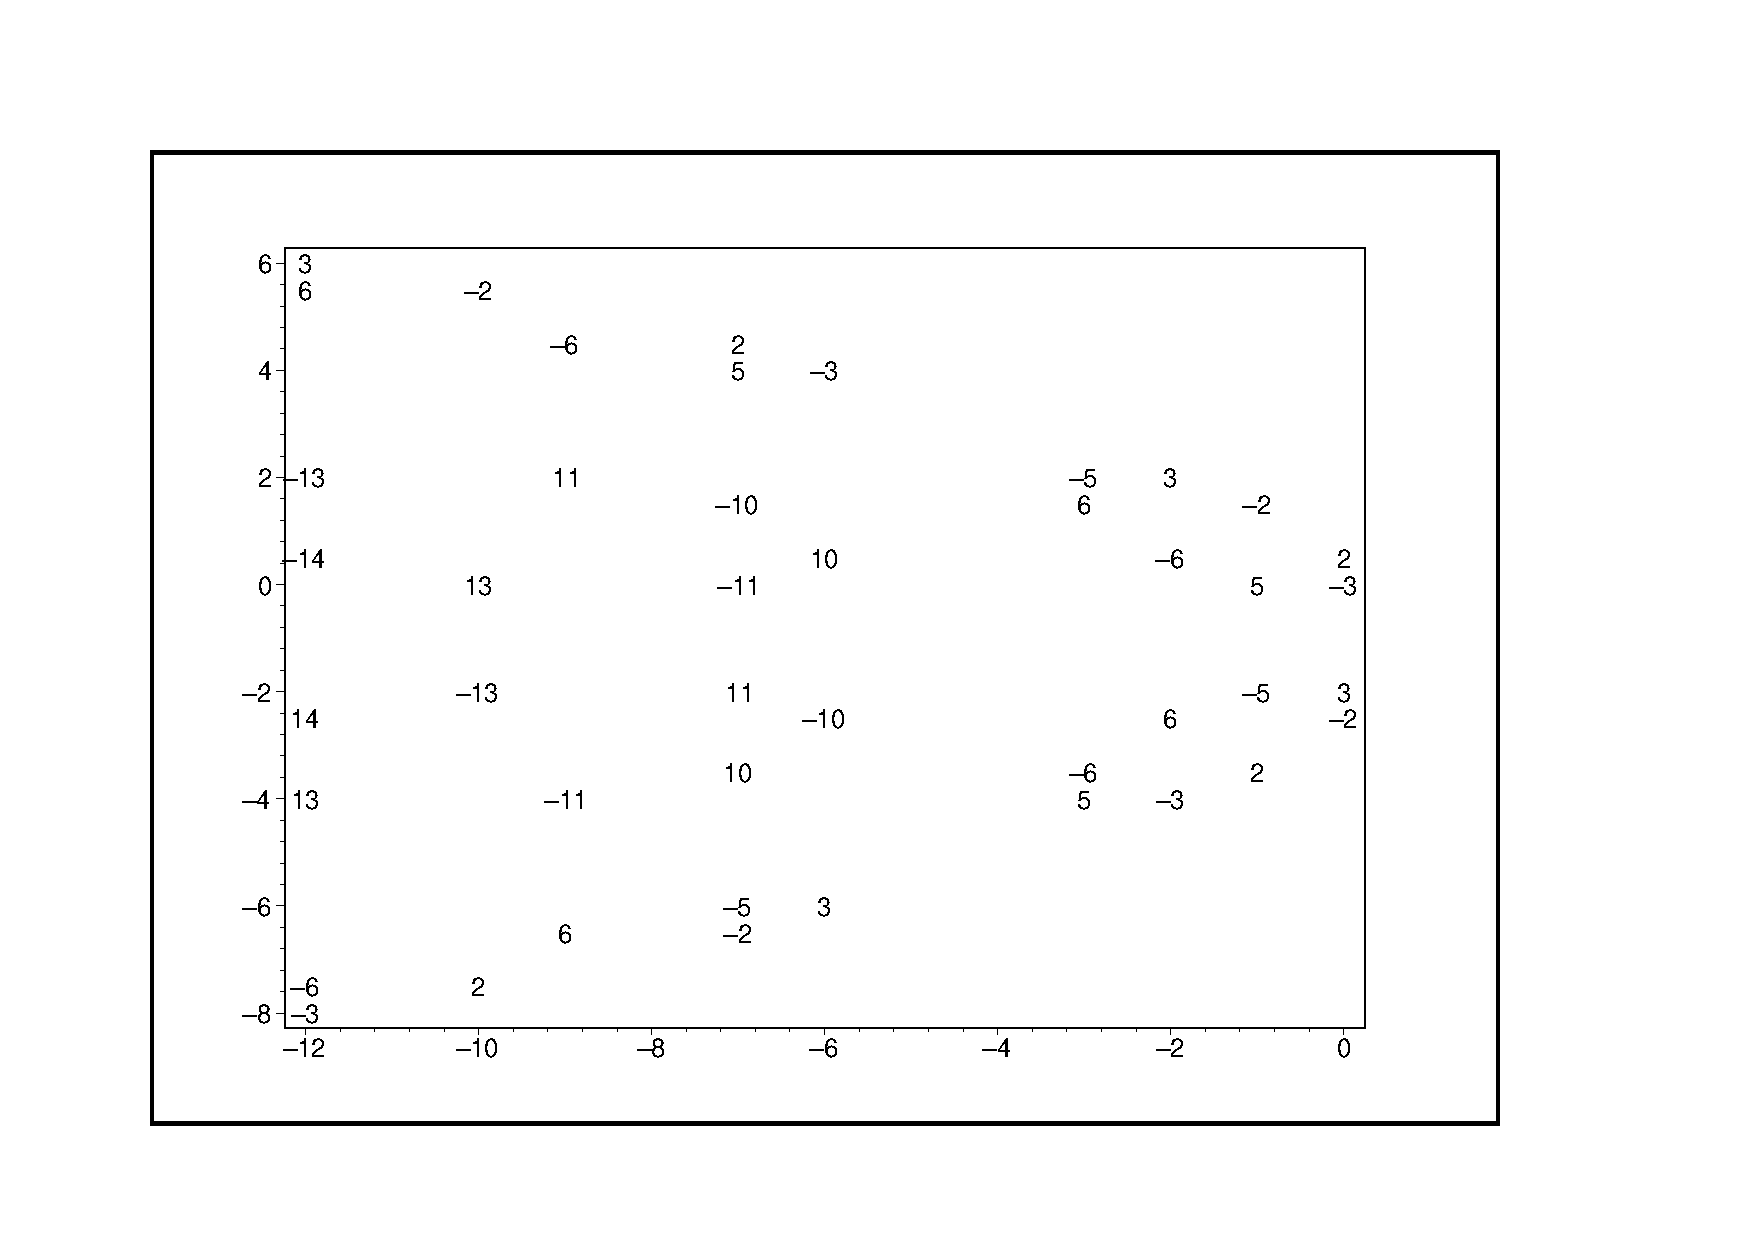
\includegraphics[width=150mm]{AffineB2_A1_proj_anom.pdf}
  \caption{Projected anomalous points and the dimensions of $\mathfrak{a}_{\bot}$-modules.}
  \label{fig:AffineB2_A1_anom_proj}
\end{figure}

Then we should construct ``the fan'' and use the recurrent relation for the computation of anomalous branching coefficients.

Using the definition (\ref{fan-defined}) we get the following set of
the points $\Gamma$ with the corresponding values $s(\gamma+\gamma_0)$: \ref{fig:AffineB2A1Fan}.
Here we restricted the computation to the twelfth grade.
\begin{figure}[ph]
  \centering
  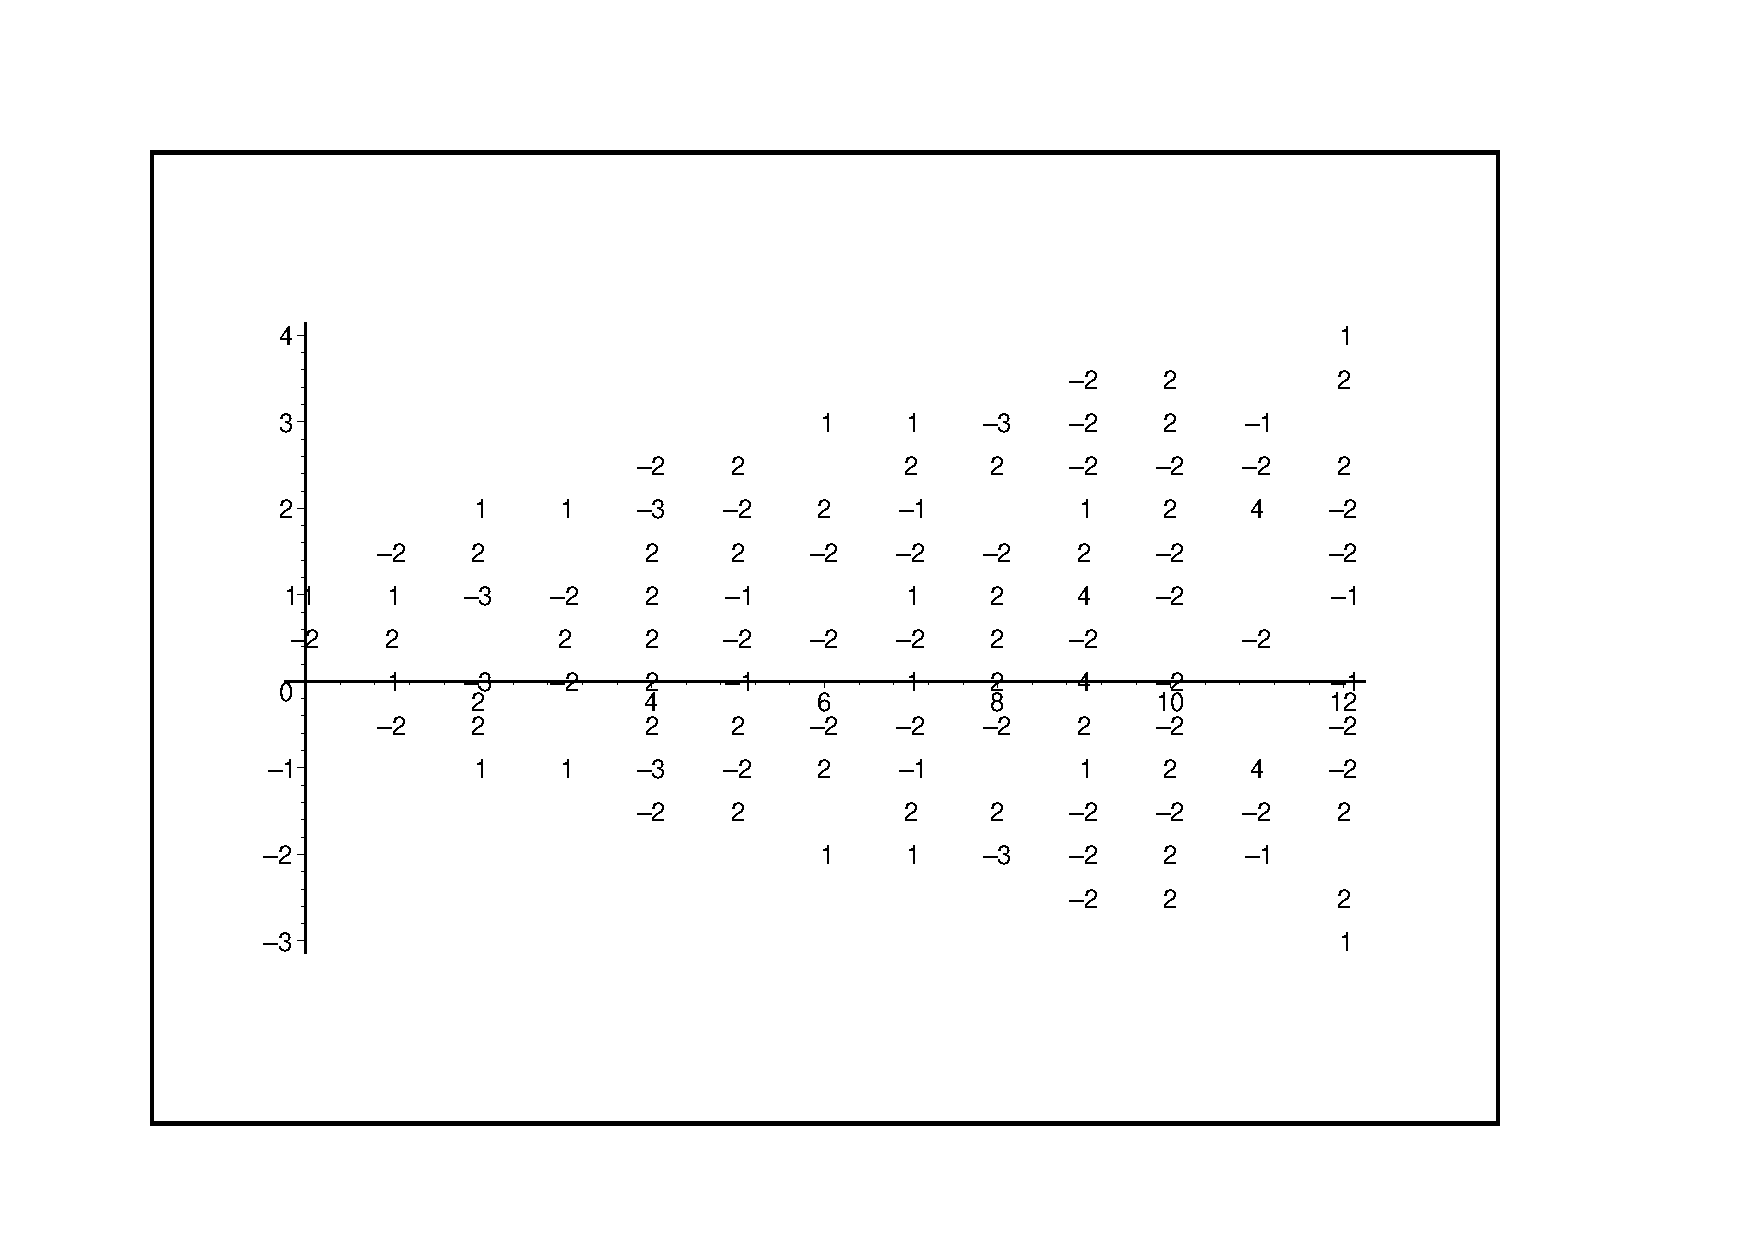
\includegraphics[width=130mm]{AffineB2_A1_fan.pdf}
  \caption{Fan for $\hat{A_1}\subset \hat{B_2}$}
  \label{fig:AffineB2A1Fan}
\end{figure}

Also we should mention that the lowest vector of the fan $\gamma_0$ is equal to zero, since we have excluded all the roots of $\Delta^{+}_{\bot}$ from the defining relation (\ref{fan-defined}).

Using the recurrent relation for the anomalous branching coefficients we get the following result
\begin{figure}[ph]
  \centering
  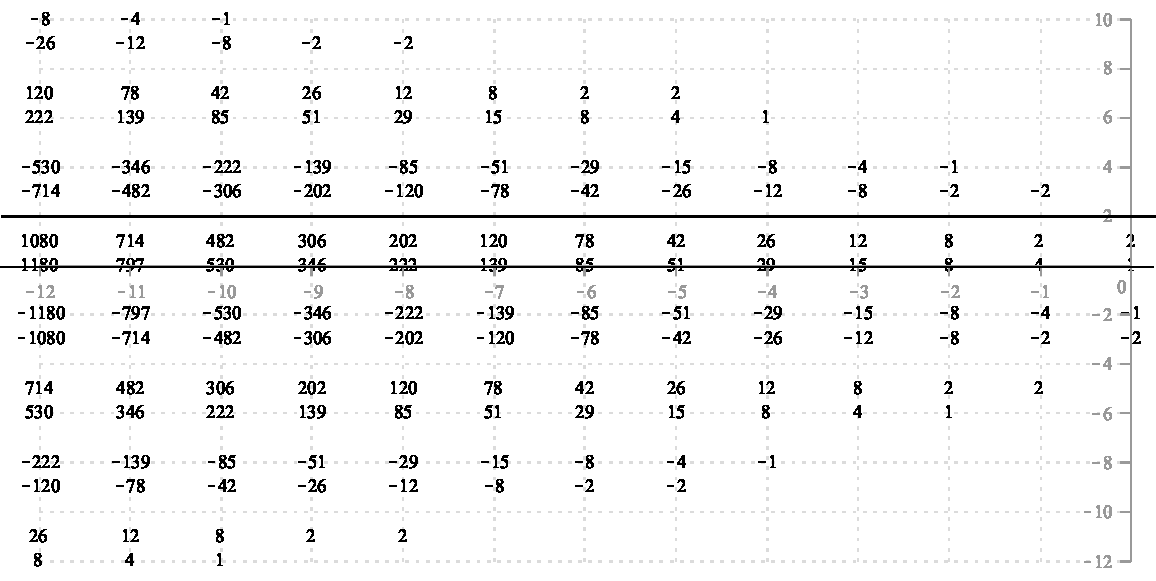
\includegraphics[width=130mm]{AffineB2_A1_branching.pdf}
  \caption{Anomalous branching coefficients for $\hat{A_1}\subset \hat{B_2}$}
  \label{fig:AffineB2_A1_branching}
\end{figure}

Selecting the points inside the main Weyl chamber of the subalgebra $\hat{A_1}$ we get the following results for the branching coefficients up to twelfth grade
\begin{multline}
  \label{eq:28}
  L^{w_1}_{\hat{B_2}\downarrow \hat{A_1}}=2 L_{\hat{A_1}}^{w_1}(0)\oplus 1 L_{\hat{A_1}}^{w_0}(0)\oplus 4 L_{\hat{A_1}}^{w_0}(-1)\oplus\\
    2 L_{\hat{A_1}}^{w_1}(-1)\oplus 8 L_{\hat{A_1}}^{w_0}(-2)\oplus
    8 L_{\hat{A_1}}^{w_1}(-2)\oplus 15 L_{\hat{A_1}}^{w_0}(-3)\oplus\\
    12 L_{\hat{A_1}}^{w_1}(-3)\oplus 26 L_{\hat{A_1}}^{w_1}(-4)\oplus
    29 L_{\hat{A_1}}^{w_0}(-4)\oplus 51 L_{\hat{A_1}}^{w_0}(-5)\oplus\\
    42 L_{\hat{A_1}}^{w_1}(-5)\oplus 78 L_{\hat{A_1}}^{w_1}(-6)\oplus
    85 L_{\hat{A_1}}^{w_0}(-6)\oplus 120 L_{\hat{A_1}}^{w_1}(-7)\oplus\\
    139 L_{\hat{A_1}}^{w_0}(-7)\oplus 202 L_{\hat{A_1}}^{w_1}(-8)\oplus
    222 L_{\hat{A_1}}^{w_0}(-8)\oplus 306 L_{\hat{A_1}}^{w_1}(-9)\oplus\\
    346 L_{\hat{A_1}}^{w_0}(-9)\oplus 530 L_{\hat{A_1}}^{w_0}(-10)\oplus
    482 L_{\hat{A_1}}^{w_1}(-10)\oplus 714 L_{\hat{A_1}}^{w_1}(-11)\oplus\\
    797 L_{\hat{A_1}}^{w_0}(-11)\oplus 1080 L_{\hat{A_1}}^{w_1}(-12)\oplus
    1180 L_{\hat{A_1}}^{w_0}(-12)
\end{multline}
This result can be expressed using the power series expansion of the branching functions \cite{kac1990idl}.
\begin{eqnarray}
  \label{eq:29}
  \begin{array}{cc}
    b^{(w_1)}_{0}= & 1 + 4\,q^{1}+ 8\,q^{2}+ 15\,q^{3}+ 29\,q^{4}+ 51\,q^{5}+ 85\,q^{6}+ 139\,q^{7}+\\
     &222\,q^{8}+ 346\,q^{9}+ 530\,q^{10}+ 797\,q^{11}+ 1180\,q^{12}+\dots\\
  \end{array}\\
  \begin{array}{cc}
    b^{(w_1)}_{1}= &2+2\,q^{1}+8\,q^{2}+12\,q^{3}+26\,q^{4}+42\,q^{5}+78\,q^{6}+120\,q^{7}+\\
    & 202\,q^{8}+306\,q^{9}+482\,q^{10}+714\,q^{11}+1080\,q^{12}+\dots
  \end{array}
\end{eqnarray}
Here the lower index of the branching function denotes the number of the corresponding $\hat{A_1}$ fundamental weight $w_0=\lambda_0=(0,1,0),\; w_1=\alpha/2=(1,1,0)$.

\newpage
\section{Physical applications}
\label{sec:phys-appl}
Here we want to discuss possible applications of the described techniques in physical models. 

Branching coefficients for the embedding of affine Lie subalgebra into
affine Lie algebra can be used to construct modular invariant
partition functions of Wess-Zumino-Novikov-Witten models (\cite{difrancesco1997cft}, \cite{Walton:1999xc}, \cite{walton1989conformal}, \cite{schellekens1986conformal}). 

But for this construction to work the embedding is required to be conformal, which means that the central charge of the subalgebra is equal to the central charge of the algebra.
\begin{equation}
  \label{eq:31}
  c(\mathfrak{a})=c(\mathfrak{g})
\end{equation}

 The class of the conformal embeddings is rather small, the complete classification is given in the paper \cite{schellekens1986conformal}. 
The requirement (\ref{eq:31}) allows to reduce the task of the computation of the branching coefficients of affine Lie algebras to the computation of the branching coefficients of the finite-dimensional Lie algebras.

Here we describe this procedure and discuss how the requirement (\ref{eq:31}) can be used to simplify the algorithm \ref{sec:algorithm}.

\begin{comment}
  Change ``enveloping'' into something better.
\end{comment}
Conformal embeddings should preserve conformal invariance, so Sugawara central charge should be the same for enveloping and embedded theory. 

The states for the theory that corresponds to the algebra $\mathfrak{g}$
\begin{equation}
  \label{eq:109}
  J^{a_1}_{-n_1}J^{a_2}_{-n_2}\dots\left|\lambda\right>\quad n_1\geq n_2\geq\dots>0
\end{equation}
For sub-algebra $\mathfrak{a}\subset\mathfrak{g}$
\begin{equation}
  \label{eq:110}
  \tilde{J}^{a'_1}_{-n_1}\tilde{J}^{a'_2}_{-n_2}\dots\left|\pi_{\mathfrak{a}}(\lambda)\right>
\end{equation}
Here $\tilde{J}^{a'_j}_{-n_j}$ are the generators of $\mathfrak{a}$ and $\pi_{\mathfrak{a}}$ is the projection of $\mathfrak{g}$ to $\mathfrak{a}$. $\mathfrak{g}$-invariance of vacuum entails its $\mathfrak{a}$-invariance, but it is not the case for energy-momentum tensor. So energy-momentum tensor of bigger theory should consist only of generators of $\mathfrak{a}$. Then $T_{\mathfrak{g}}=T_{\mathfrak{a}}\Rightarrow c(\mathfrak{g})=c(\mathfrak{a})$. This leads to equation
\begin{equation}
  \label{eq:111}
  \frac{k\;\mathrm{dim}\,\mathfrak{g}}{k+g}=\frac{x_e k\; \mathrm{dim}\,\mathfrak{a}}{x_ek+a}
\end{equation}
Here $x_e$ is the embedding index and $g$, $a$ are dual Coxeter numbers of corresponding algebras. 

It can be shown that solutions of equation (\ref{eq:111}) exist only
for level 1 $k=1$ \cite{difrancesco1997cft}.

If we have modular-invariant partition function for the fields described by the representation of the algebra $\mathfrak{g}$ this modular invariance is preserved by the projection on the subalgebra $\mathfrak{a}$, but we need also the preservation of the conformal invariance. So we should select only those highest-weight modules of the subalgebra $\mathfrak{a}$ for which the relation (\ref{eq:111}) holds.

Since in the decomposition (\ref{eq:3}) the highest weight $\nu$ of the subalgebra module belongs to some grade $n$ of projected algebra module $\pi_{\mathfrak{a}}\cdot L^{(\mu)}_{\mathfrak{g}}$, from the relation (\ref{eq:111}) one can obtain the following requirement on the conformal dimensions of the corresponding fields
\begin{equation}
  \label{eq:32}
   \Delta_{\pi_{\mathfrak{a}}\mu}+n=\Delta_{\nu}
\end{equation}
It leads to the relation on the classical parts of the corresponding weights:
\begin{equation}
  \label{eq:33}
  \frac{(\overset{\circ }{\mu},\overset{\circ }{\mu}+2\rho)}{2(1+g)}+n=\frac{(\overset{\circ }{\nu},\overset{\circ }{\nu}+2\rho_{\mathfrak{a}})}{2(x_e+a)}
\end{equation}
There exits the finite reducibility theorem for the conformal embeddings which states that only finite number of the branching coefficients is non-zero in the case of the conformal embedding $\mathfrak{a}\subset\mathfrak{a}$.

Then after we have found all such weights $\nu$ and the corresponding branching coefficients $b^{(\mu)}_{\nu}$ we can substitute the sums $\sum_{\nu \in P^{+}_{\mathfrak{a}}}b^{(\mu)}_{\nu} \chi_{\nu}$ over the modified characters $\chi_{\nu}$ of the corresponding $\mathfrak{a}$-modules in place of the characters of the $\mathfrak{g}$-modules in the diagonal modular-invariant partition function
\begin{equation}
  \label{eq:34}
   Z(\tau)=\sum_{ \mu\in P^{+}_{\mathfrak{g}}} \chi_{\mu}(\tau)\bar \chi_{\mu}(\bar \tau)
\end{equation}
Thus we obtain the non-diagonal modular-invariant  partition function for the theory with the current algebra $\mathfrak{a}$.
\begin{equation}
  \label{eq:36}
   Z_{\mathfrak{a}}(\tau)=\sum_{ \nu,\lambda\in P^{+}_{\mathfrak{a}}} \chi_{\nu}(\tau)M_{\nu\lambda}\bar \chi_{\lambda}(\bar \tau)
\end{equation}


\subsection{Example}
\label{sec:example}

Consider the level ten embedding of the affine $\hat A_1$ into the level one affine $\hat C_2$. 
The relation (\ref{eq:33}) and the finite reducibility theorem greatly simplify the calculation with the algorithm \ref{sec:algorithm}, since we know that there exists only finite number of the non-zero branching coefficients and the maximal grade of this coefficients is restricted.

This affine embedding is the affine extension of the special embedding $A_1\subset C_2$ with the embedding index equal to 10. The projection of the weights of algebra $C_2$ is calculated using the projection matrix $\mathcal{P}=(3,4)$. The embedding index
\begin{equation}
  \label{eq:37}
  x_e=\frac{\left|\mathcal{P}\Theta_{\mathfrak{g}}\right|^2}{\left|\Theta_{\mathfrak{a}}\right|^2}=\frac{k_{\mathfrak{a}}}{k_{\mathfrak{g}}}=10
\end{equation}
If we consider this embedding in the orthogonal basis where the simple roots of $C_2$ are given by
\begin{equation}
  \label{eq:38}
  \alpha_1=(1,-1),\quad \alpha_2=(0,2),
\end{equation}
then the simple root of the embedded $A_1$ is equal to
\begin{equation}
  \label{eq:39}
  \beta=\sqrt{\frac{2}{5}}(3,1)
\end{equation}
It is easy to see that the set $\Delta^{+}_{\bot}$ of the $C_2$ roots orthogonal to $\beta$ is empty.

Now we proceed the computation of the branching coefficients using the algorithm \ref{sec:algorithm}. 
On the level 1 there exist three dominant weights with Dynkin labels $[1,0,0], \; [0,1,0],\; [0,0,1]$.

\begin{comment}
  Do the calculation, show the restriction on the grade and the final result
  \begin{equation}
    \label{eq:35}
    Z=\left|\chi_{[10,0]}+\chi_{[4,6]}\right|^2+\left|\chi_{[7,3]}+\chi_{[3,7]}\right|^2+\left|\chi_{[6,4]}+\chi_{[0,10]}\right|^2
  \end{equation}
\end{comment}

\section{Conclusion}
\label{sec:conclusion}
We have proved the recurrent relation on the branching coefficients and proposed practical algorithm of the reduction of the representations. Also we have discussed the application of this algorithm to the physical problem of construction of modular-invariant partition functions in the conformal field theory. This method of conformal embeddings is well-known but may be actual in the study of WZW-models emerging in the context of the AdS/CFT correspondence \cite{Maldacena:2000hw,Maldacena:2000kv,Maldacena:2001km}. 
\begin{comment}
  What about acknowledgements? 
\end{comment}
\bibliography{article}{}
\bibliographystyle{utphys}

\end{document}
